\RequirePackage{fix-cm}
% \documentclass[12pt]{article}
\documentclass[12pt]{new-aiaa}

% Formatting
\usepackage[utf8]{inputenc}
\usepackage{hyperref}
\usepackage{graphicx}
\usepackage{siunitx}
\sisetup{group-separator = {,}}
\usepackage{booktabs}
\usepackage{enumitem}
\usepackage{float}
\usepackage{amsmath}
\usepackage[version=4]{mhchem}
\usepackage{longtable,tabularx}
\usepackage{placeins}
\usepackage{multirow}
\usepackage{booktabs}
\usepackage{latexsym}
\usepackage{subcaption}
\usepackage{latexsym}
\usepackage[sort&compress,numbers]{natbib} % For bibtex \citet, \citep
\usepackage{hypernat} % To get natbib to play nicely with hyperref
\usepackage{doi} % For getting hyperlinked DOI in the references

\graphicspath{{../figures/}}

% Title content
\title{AERO 590: Comparing Hydrogen and Jet-A for a Ultra High-Bypass Turbofan with Water Recirculation}
\author{Peter Atma}
% \affil{University of Michigan, AERO 590}

\begin{document}

\maketitle

\section{Introduction}
The effects of climate change are pushing the aviation industry towards hydrogen-fueled propulsion systems as a solution to reduce emissions.
N+3 technology estimates for turbofan engines that burn hydrocarbon fuels suggest that higher efficiency can be achieved by designing ultra high-bypass (UHB) engines with small cores and high overall pressure ratios (OPR).
Higher OPR and smaller cores are pushing the limits of compressor and turbine design, placing an upper bound on potential performance and emissions improvements.
Switching to hydrogen as the primary fuel source reduces carbon dioxide emissions immediately, but adds complexity and weight that offset the benefits.
However, hydrogen is a versatile fuel with advantageous chemical and thermodynamic properties that can be leveraged to further increase the performance and emission reduction of the propulsion system.
In this study, we investigate the tradeoff between burning hydrocarbon fuels like Jet-A versus hydrogen for UHB ratio turbofan engines.
We will look at new ideas with water recirculation to further squeeze performance and efficiency from Jet-A and hydrogen combustion using gradient-based design optimization.

Water recirculation is the process of extracting water from the exhaust stream of a propulsion system and injecting it upstream of the combustor as finely atomized droplets.
NASA, Boeing, and Rolls-Royce studied injectiong water into the airstream and suggested that this technique reduces the NOx emissions as much as 47 percent~\cite{nasa_inject}.
Additionally, water recirculation improves fuel efficiency and thrust output with lower burner temperatures that can improve the lifetime of turbine blades and reduce noise~\cite{nasa_inject}.
Traditional propulsion systems that burn hydrocarbon fuels would require external water storage on the aircraft because they do not produce enough in the exhaust for recirculation.
The added weight of tanks, pumping, and ducting makes this concept infeasible for a conventional aircraft.
However, if hydrogen fuels are used, the main product of hydrogen combustion is water vapor and can thus be recovered.
The ability to recirculate water vapor from the exhaust of hydrogen combustion reduces the requirement for storage tanks and allows for the creation of a closed loop system inside the propulsion cycle.
Additionally, Pratt and Whitney are currently looking at closed-loop water vapor recovery for impementation in their Hydrogen Steam-Injected, Inter‐Cooled Turbine Engine (HySIITE) as part of the US Departement of Energy's Advanced Research Projects Agency-Energy (ARPA-E) program \cite{hysiite}.
Pratt and Whitney suggest that this type of hydrogen-powered engine could achieve zero-carbon emissions and reduce NOx emissions by as much as 80\%.

Zero-dimensional cycle modeling is an efficient tool for predicting the initial design, performance, and emissions of new propulsion concepts.
Zero-dimensional cycle analysis uses a first-principles approach with a chemical equilibrium analysis (CEA) thermodynamics solver that considers the molecular species of different fuels.
This can be used to understand the trends and design limitations of an engine cycle and study potential improvements in design using optimization.
The industry standard for zero and one-dimensional cycle analysis is the Numerical Proprulsion System Simulation (NPSS) framework~\cite{JonesNPSS}.
NPSS is a modular object-oriented framework that models engine components as individual blocks with several thermodynamic solvers.
\citet{Hendricks2019} and \citet{Gray2017b} created a tool called pyCycle with the same functionality as NPSS, but includes analytical derivatives for each engine component and thermodynamic solver.
We use pyCycle because it is built on top of the OpenMDAO framework~\cite{Gray2019a} to simplify gradient-based optimization and leverage hierarchical nonlinear solver structures for robustness.

In this work, the potential propulsion benefits of a closed-loop water vapor recovery and water injection system are analyzed in a high-bypass turbofan engine by optimizing the thrust-specific energy consumption (TSEC).
TSEC is the thrust specific fuel consumption multiplied by the lower heating value of the fuel and is a metric for comparing the efficiency of different fuel choices.
New pyCycle components are developed for water injection and vapor recovery within pyCycle to understand the benefit of a closed loop recirculation system.

\section{Model}

\subsection{Engine Model Overview}
The engine model that was selected for this project is the NASA advanced technology UHB geared turbofan engine cycle, referred to as the "N+3" engine \cite{Jones2017a}.
The N+3 reference cycle represents a UHB ratio geared turbofan that could be available in the 2030–2040 time frame and was selected since it has already been modeled in pyCycle as a robust example cycle and includes the advanced engine cycle improvements such as a large bypass ratio, high pressure ratio, and high combustion temperature.
The flow path consists of an inlet that directs ambient air through a fan, followed by a duct that splits the flow into a core flow and a bypass flow, each of which ends in a bypass nozzle and core nozzle, respectively.
The fan and low pressure compressor (LPC) are connected to the low pressure turbine (LPT) by the low pressure shaft and the high pressure compressor (HPC) is connected to the high pressure turbine (HPT) by the high pressure shaft.
Along the axial flow path, the zero-dimensional thermodynamic connections are solved using CEA to ensure first the principle governing equations are satisfied.
Figure \ref{fig:N3_original} shows how the 25 elements in the N+3 cycle are connected together with the fluid flows in blue, the mechanical connections in red, and the performance elements in green.

\begin{figure}[!hbt]
    \centering
    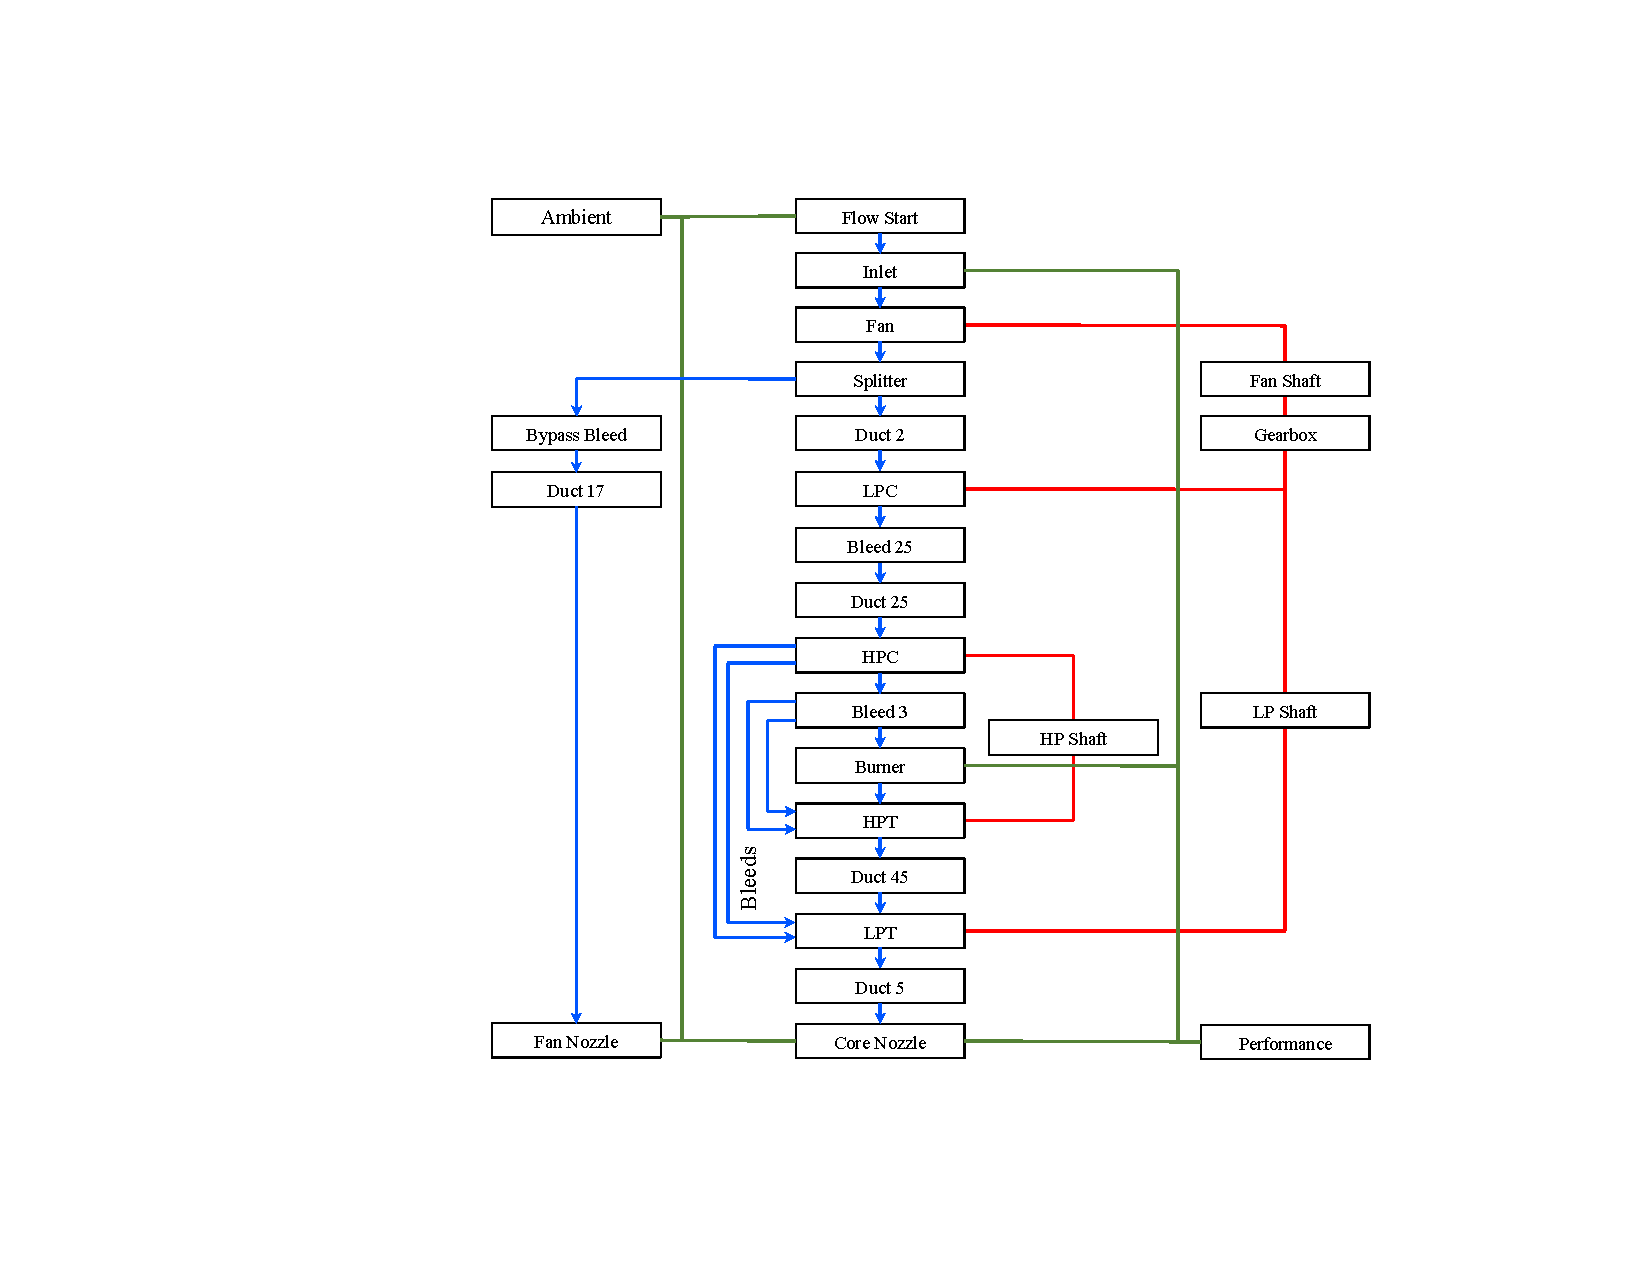
\includegraphics[width=0.75\textwidth]{N3_diagram.pdf}
    \caption{N+3 cycle layout.}
    \label{fig:N3_original}
\end{figure}

\noindent
The N3 engine model as it is implemented in pyCycle has many complex thermodynamic and performance connections between different operating conditions.
These operating conditions are top-of-climb (TOC), rotating takeoff (RTO), sea-level static (SLS), and cruise (CRZ).
To account for each of these operating conditions, the N3 model uses a technique called Multipoint Design Point (MDP) modeling to converge to an engine design that satisfies the requirements at each of these operation conditions.
One of the operation conditions is specified as the design point which in this case is TOC and the other operating conditions are the off-design points.
The design point of the engine model is converged using a linear Newton solver which then passes the geometric sizing variables to the off-design points and similarly converges those.
Then, a nonlinear Newton solver is used to converge the overall model with respect to the variable connections between each point.
An XDSM diagram of the nominal N3 engine model is shown in Figure \ref{fig:N3_xdsm}.

\begin{figure}[!hbt]
    \centering
    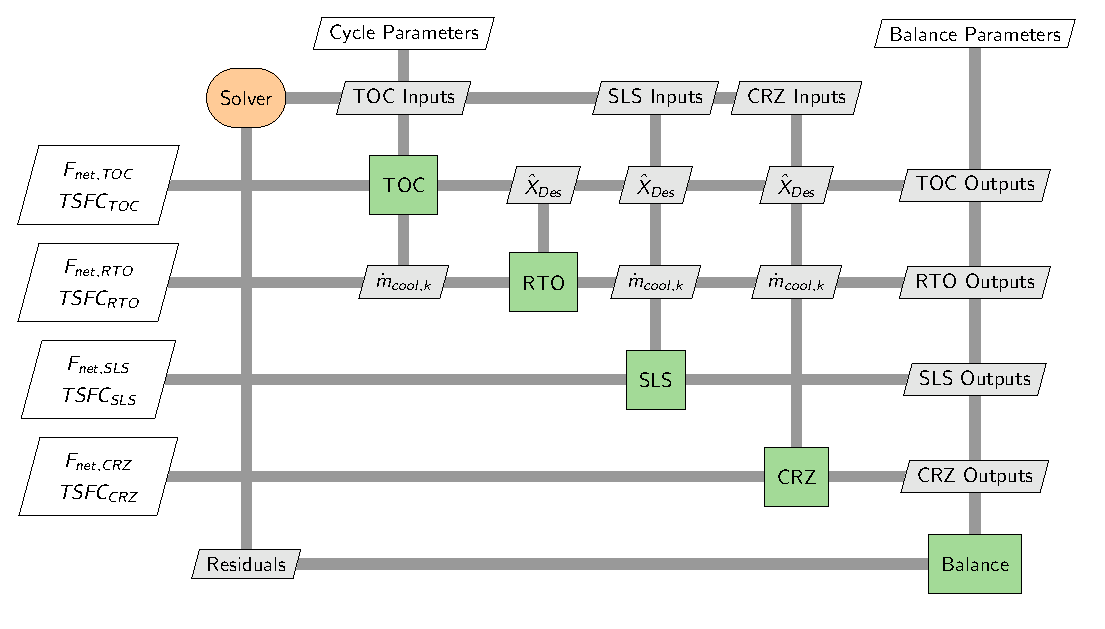
\includegraphics[width=0.75\textwidth]{N3_xdsm.pdf}
    \caption{N+3 Multipoint XDSM diagram.}
    \label{fig:N3_xdsm}
\end{figure}

\subsection{Water Recovery Model}
The closed-loop water recovery system is implemented into the cycle by placing a water injection component directly before the HPC.
This component will inject pure water into the core stream which will reduce the combustion temperature due to heat absorption from vaporization.
This location was chosen as it was one of the configurations chosen by the afformetioned NASA, Boeing, and Rolls-Royce study that did not require direct combustor injection \cite{nasa_inject}.
The water vapor recovery component is placed directly before the core nozzle to extract water from the core stream and recycle it back to the water injector.
Water is recovered from this location as it is the last possible location before the nozzle in which water can be extracted.
In practice a water vapor recovery component requires a complex condenser model in the core stream, this work will only look at the potential benefits of extracting water vapor and not the recovery method specifically.
The component flow interface and mechanical connections, including the water injector and water extractor, are depicted in Figure \ref{fig:hbtf_cycle}.

\begin{figure}[!hbt]
    \centering
    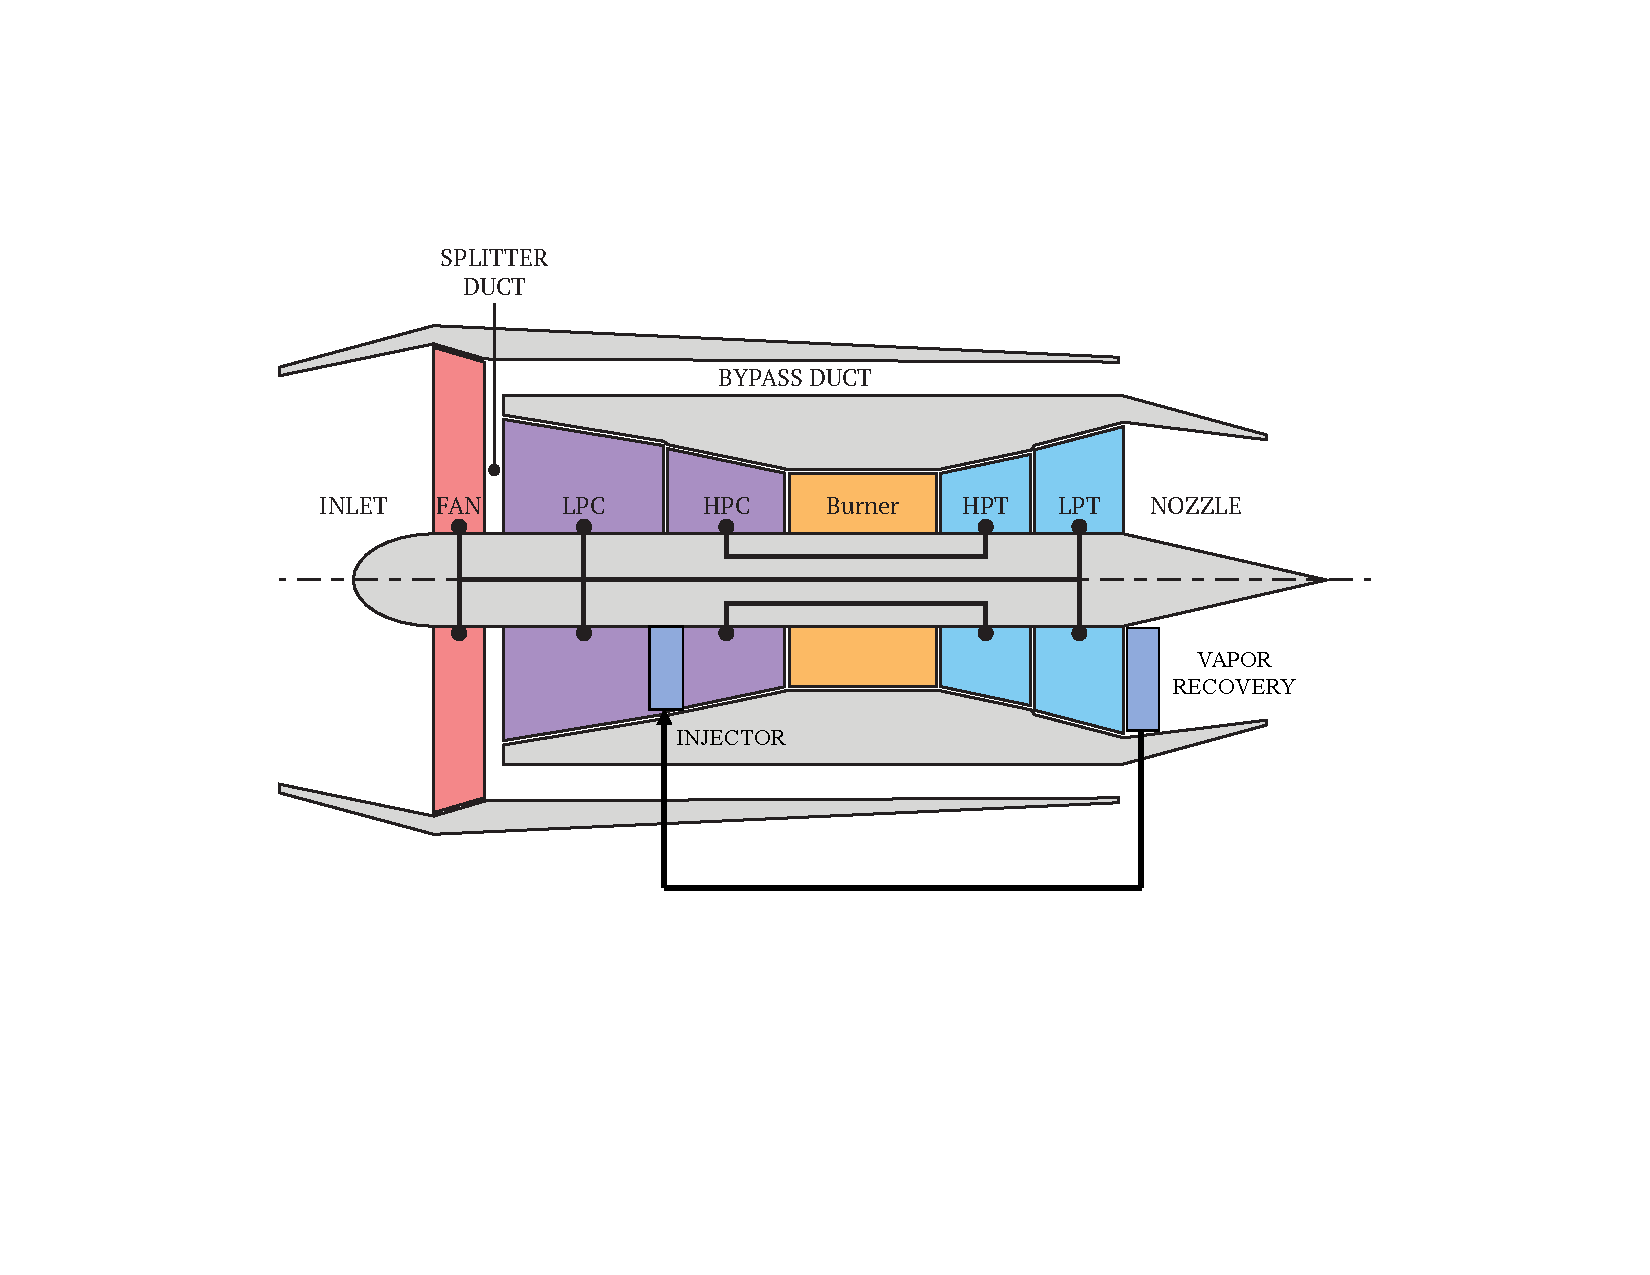
\includegraphics[width=0.75\textwidth]{turbofan_wvr.pdf}
    \caption{The configuration of a high-bypass turbofan model with an integrated closed-loop water vapor recovery and injection system.}
    \label{fig:hbtf_cycle}
\end{figure}

\noindent
To model this complicated water recirculation loop in pyCycle new components had to be developed.
The two new components that were developed are a water injector to add water to the flow and a water extractor to divert a fraction of the water in the flow back upstream.
The injector component is based on the combustor component already included in pyCycle which operates by injecting a given fuel-to-air ratio (FAR) or fuel flow rate to determine the mass of fuel added to the incoming flow.
This new mixture combination is then used to compute the various chemical species present in the flow at the given thermodynamic state which is determined by the incoming flow.
The new species composition and thermodynamic variables are then determined using a Gibbs Free Energy minization approach called Chemical Equilibrium with Applications (CEA).
Once the new composition is determined, the various thermodynamic variables are passed to the next component in the engine.
The water injector component was created to work similarly to the combustor but would instead inject water as a reactant instead of the fuel.
The water injector can take either water-to-air ratio (WAR) or water mass flow rate to determine how much water is added to the flow.
A simple schematic of the injector is shown in Figure \ref{fig:injector} where $Y_{H_2O}$ is the mole fraction of water molecules.

\begin{figure}[!hbt]
    \centering
    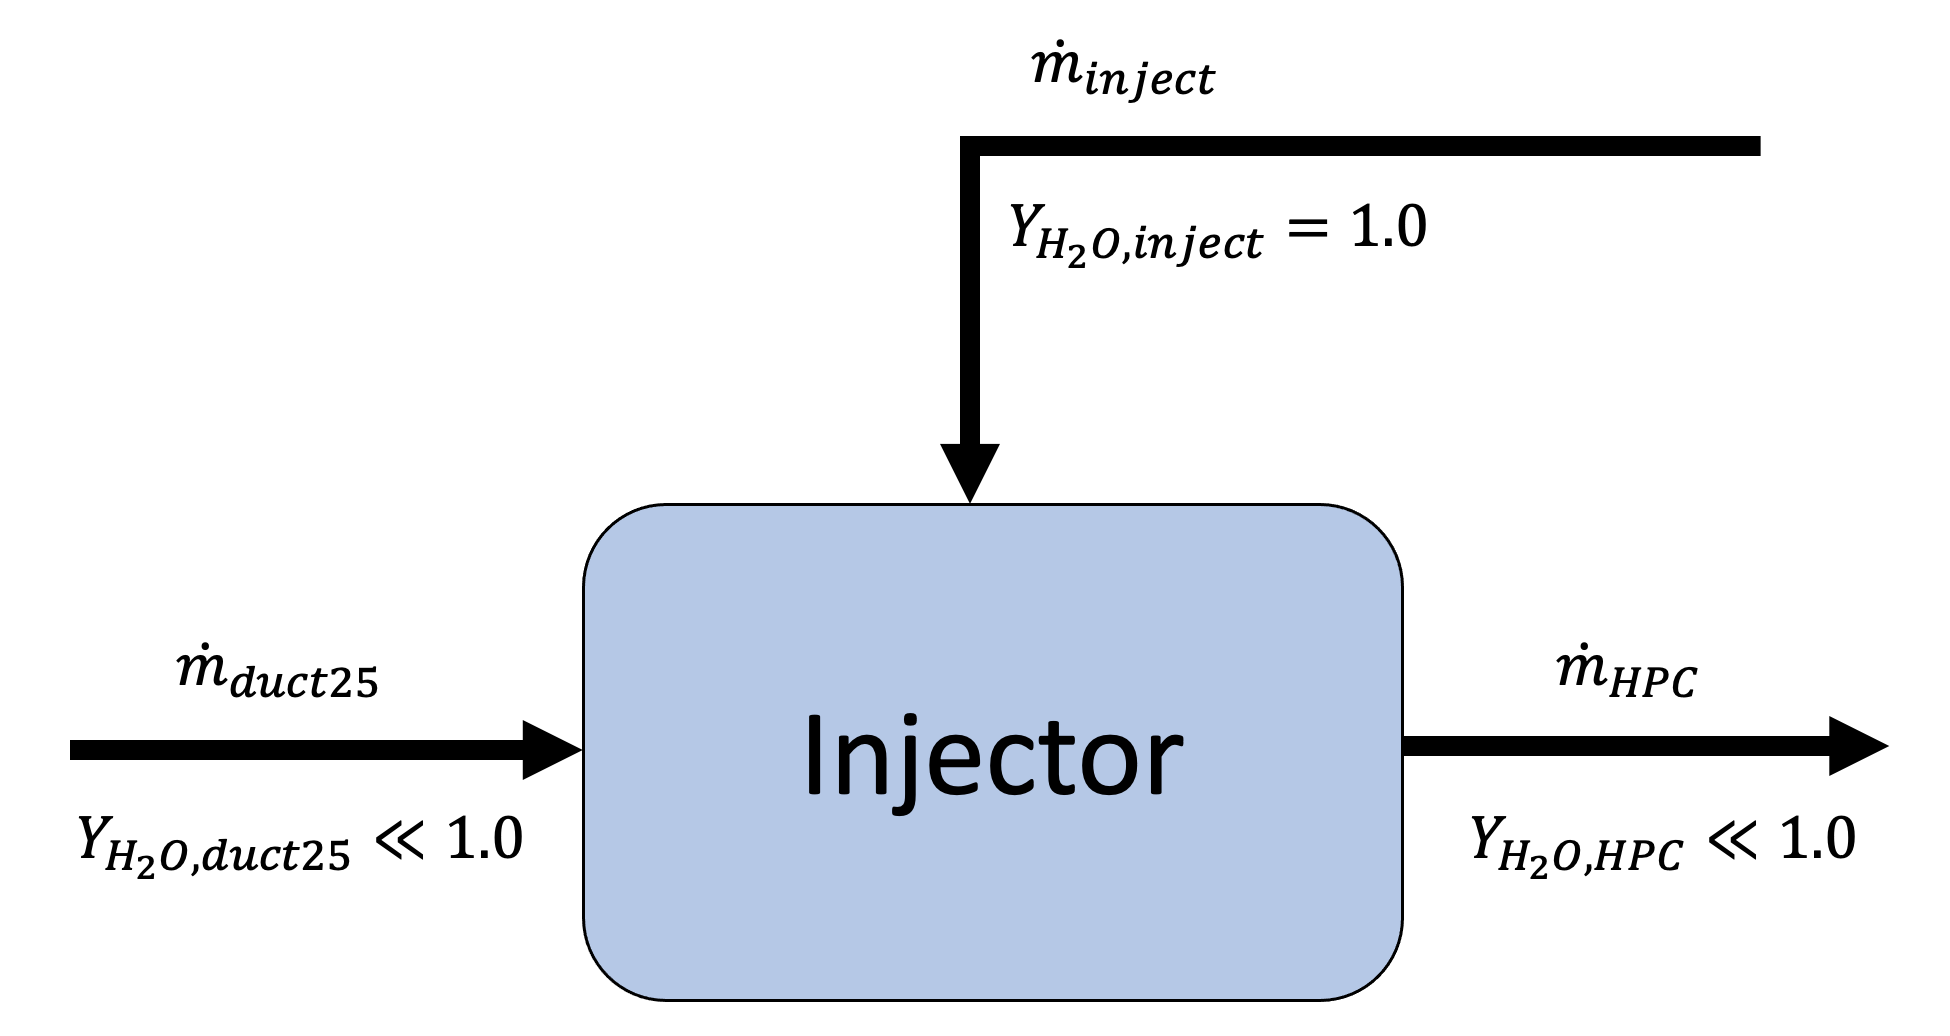
\includegraphics[width=0.75\textwidth]{injector.png}
    \caption{Injector component schematic.}
    \label{fig:injector}
\end{figure}

\noindent
The water extractor component is based on an air-bleed component in pyCycle with the added complexity of extracting a fraction of a specific species within the flow.
This extractor component works by first determining the water content of the incoming flow and extracting a given fraction of that water flow.
The water content of the incoming flow is determined by solving a CEA analysis of the incoming flow.
This water content in the incoming flow is then used with a given fraction of the water to extract to determine the how much mass flow to remove from the stream.
At the some time, the atomic mixture is updated to represent the mixture that would be left if a number of hydrogen and oxygen atoms corresponding to the amount of water were removed.
The outputs of the extractor component are the flow rate of the main flow and the corresponding properties in addition to a water mass flow rate.
While this process certainly would have pressure loss penalties in terms of condensing water in a condersor, this project looks to just look at the effects of water recovery since there are no current models for nozzle exhaust condensors.
A simple schematic of the extractor is shown in Figure \ref{fig:extractor} where $Y_{H_2O}$ is the mole fraction of water molecules and $X_{H_2O,k}$ is the fraction of water that is recovered from the core stream of operating condition, $k$.

\begin{figure}[!hbt]
    \centering
    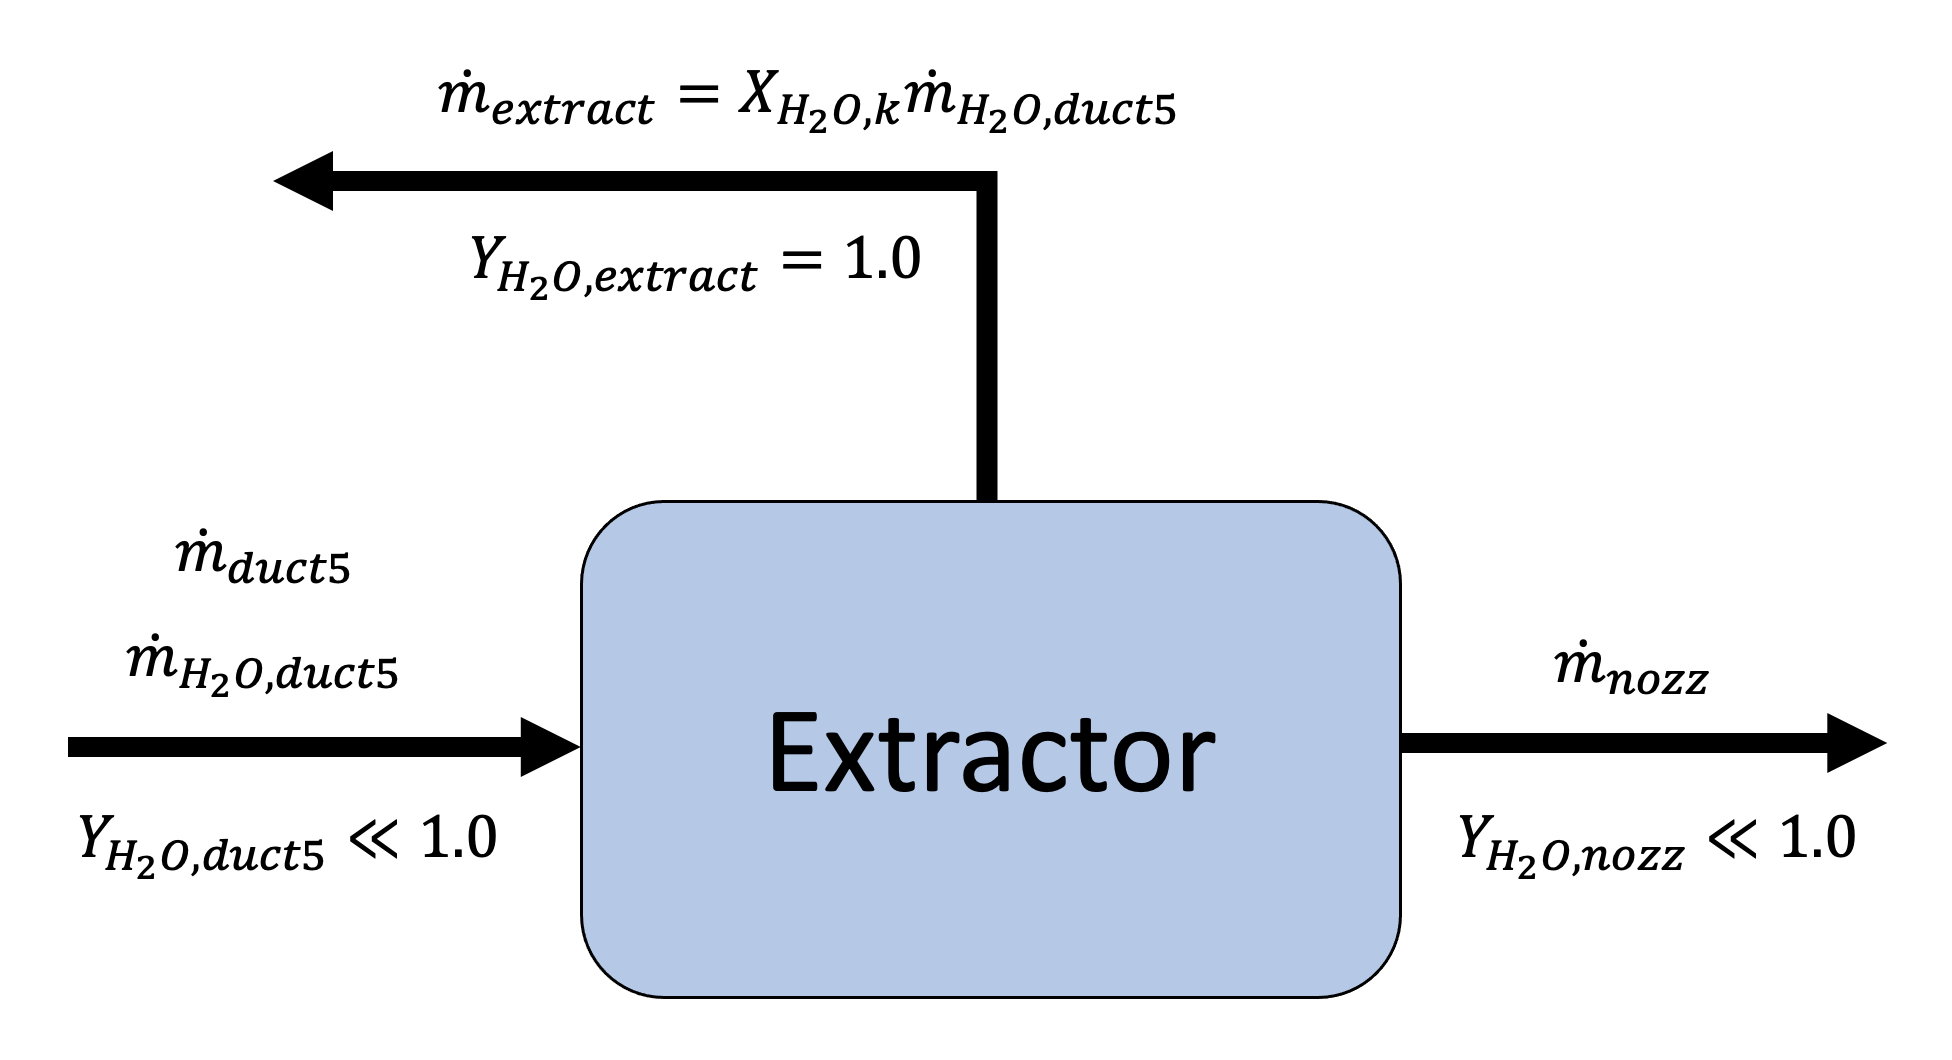
\includegraphics[width=0.75\textwidth]{extractor.png}
    \caption{Extractor component schematic.}
    \label{fig:extractor}
\end{figure}

\noindent
Unlike other flow streams in the N3 model, the vapor recovery loop would be adding a mass flow rate at the injector and extracting a mass flow rate at the extractor, the loop would have a feedback effect.
This is because the pyCycle model is solved sequentially during each Newton iteration.
So a Nonlinear Block Gauss-Seidel solver would be sufficient to solve this feedback loop.
However, the N3 model already has a nonlinear Newton solver at the Multipoint Design level, so the extractor mass flow rate and injector mass flow rate variables are connected for each design point and use this nonlinear solver to converge the water streams.
These connections can be seen in Figure \ref{fig:N3_xdsm_full}

\subsection{NOx Model}
To compute the Nitrogen Oxide (NOx) emissions from the engine model when using JetA as a fuel, the P3T3 NOx correlation was used \cite{Voet2021}.
The P3T3 method computes the NOx emission index (EINOx) of an engine at a specific operation condition as a function of the combustor pressure ($P_3$) and FAR.
The P3T3 method uses the EINOx level at sea-level operating condition as a reference point to scale the desired operating condition EINOx.
Finally, the EINOx level is scaled by a humidity factor based on the water content of the specific operating condition compared to the sea-level water content.
The P3T3 method is give below:

\begin{equation}
    EINOx_{alt} = EINOx_{SLS} \left(\frac{P_{3,alt}}{P_{3,SLS}}\right)^n \left(\frac{FAR_{alt}}{FAR_{SLS}}\right)^m e^{H}
\end{equation}

\begin{equation}
    H = 19 (h_{SLS} - h_{alt})
\end{equation}

\noindent
Experiments have shown that $n=0.4$ and $m=0$ so the FAR essentially drops out (CITE).
The sea-level EINOx level is determined using a curve-fit based on combustor inlet temperature ($T_3)$ (CITE).
The EINOx level is based on the CFM56-5B3 engine and is assumed to be proportional to $P_3^{0.4}$.

\begin{equation}
    EINOx = P_3^{0.4} (6.26 \times 10^{-8}T_3^3 - 0.000117 T_3^2 + 0.074 T_3 - 15.04)
\end{equation}

\noindent
Since the experimental data for these curve-fits are based on the CFM56-5B3 engine which runs on Jet-A fuel, this EINOx correlation will only be valid for Jet-A NOx emissions modeling.
Note, the curve-fit found in the above paper has a typo in that the factor on $T_3^2$ was $0.00117$.
However, inserting a 0 seems to fit the data curve-fit included in the paper relatively well.

\subsection{Performance Metrics}
For measuring the efficiency of jet engines, thrust-specific fuel consumption (TSFC) is generally used since is a metric of how low the fuel burn is for a given level of thrust.
However, when comparing Jet-A and hydrogen fuels this is not such a good metric since a given mass flow rate of hydrogen has an energy content almost 3 times that of Jet-A.
Therefore, a new metric for comparing the relative efficiencies of engine running on Jet-A versus hydrogen is thrust-specific energy consumption (TSEC):

\begin{equation}
    TSFC = \frac{\Dot{m}_{fuel}}{F_{thrust}}
\end{equation}

\begin{equation}
    TSEC = \frac{\Dot{m}_{fuel} LHV}{F_{thrust}} = TSFC \times LHV
\end{equation}

\noindent
With all of the sub-models of the N3 engine presented, the complete engine cycle XDSM diagram is shown in Figure \ref{fig:N3_xdsm_full} and a N2 diagram of the model shown in Figure \ref{fig:N3_n2}.

\begin{figure}[!hbt]
    \centering
    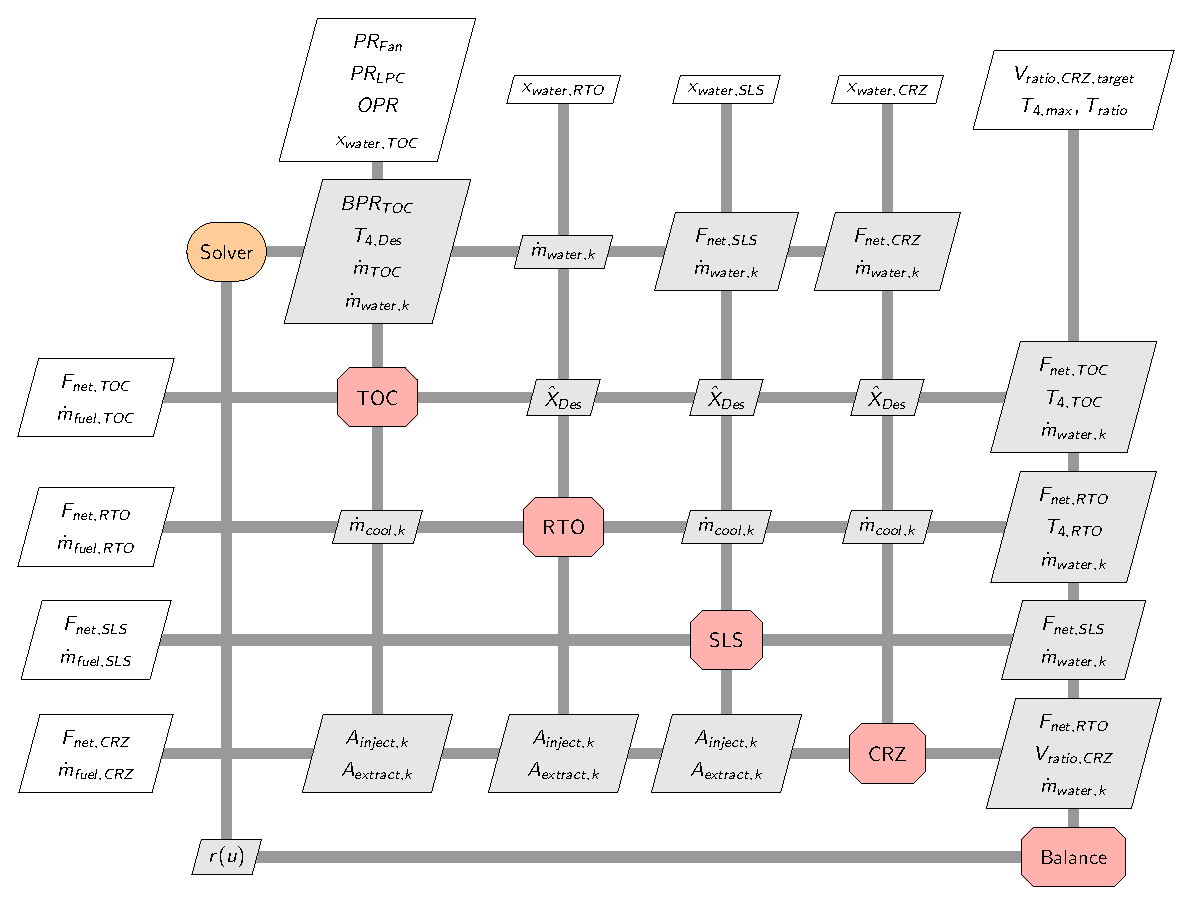
\includegraphics[width=0.75\textwidth]{N3_xdsm_full.pdf}
    \caption{Full project N+3 XDSM diagram.}
    \label{fig:N3_xdsm_full}
\end{figure}

\begin{figure}[!hbt]
    \centering
    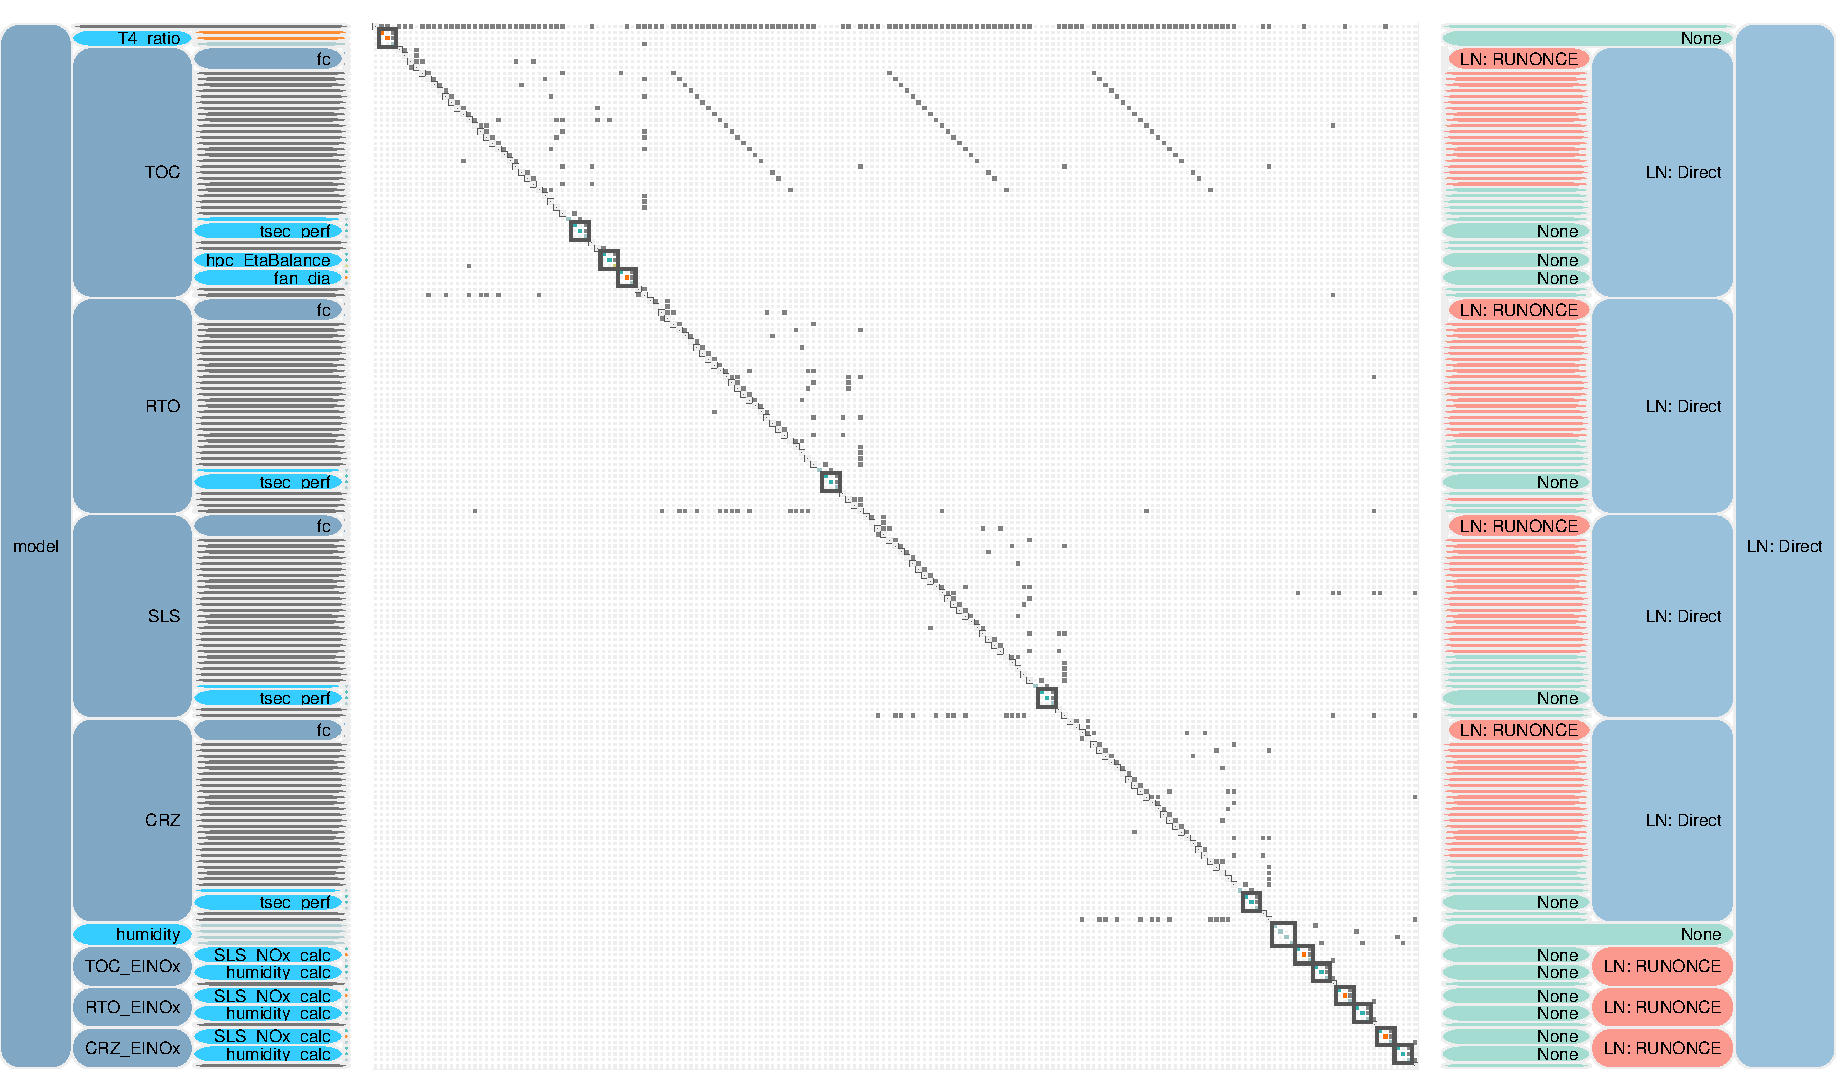
\includegraphics[width=0.75\textwidth]{N3_CLVR_n2.pdf}
    \caption{N2 diagram of the model.}
    \label{fig:N3_n2}
\end{figure}

\subsection{Model Parametric Studies}
To understand the coupling between the various operation conditions and design point, some simple parametric studies of the water recovery fraction were run.
The constant parameters for the engine and NOx model are shown in the table below.

\begin{table}[H]
    \centering
    \caption{atmosphere parameters for the parametric study.}
    \begin{tabular}{|c|c|c|c|}
        \hline
        Parameter             & Value    & Units                 & Comments \\
        \hline
        $W_{TOC}$             & 820.441  & $lbm/s$               &          \\
        $BPR_{TOC}$           & 23.945   & $-$                   &          \\
        $PR_{HPC,TOC}$        & 53.633   & $-$                   &          \\
        $PR_{LPC,TOC}$        & 3.00     & $-$                   &          \\
        $PR_{fan,TOC}$        & 1.30     & $-$                   &          \\
        $F_{net,SLS}$         & 28620.84 & $lbf$                 &          \\
        $F_{net,CRZ}$         & 5510.72  & $lbf$                 &          \\
        $T_{4,TOC}/T_{4,RTO}$ & 0.926    & $-$                   &          \\
        $T_{4,RTO}$           & 3400.0   & $R$                   &          \\
        $h_TOC$               & 0.007    & $kg_{water}/kg_{air}$ &          \\
        $h_RTO$               & 0.001    & $kg_{water}/kg_{air}$ &          \\
        $h_SLS$               & 0.001    & $kg_{water}/kg_{air}$ &          \\
        $h_CRZ$               & 0.007    & $kg_{water}/kg_{air}$ &          \\
        $n$                   & 0.4      & $-$                   &          \\
        $m$                   & 0.0      & $-$                   &          \\
        \hline
    \end{tabular}
    \label{hx_params}
\end{table}

\noindent
Each of the 4 water recovery fractions was varied independently of the other 3 to gain an understanding of how that particular point was coupled with the rest.
The results are shown in Figure \ref{fig:para_study}.

\begin{figure}[!hbt]
    \centering
    \begin{minipage}{0.48\textwidth}
        \centering
        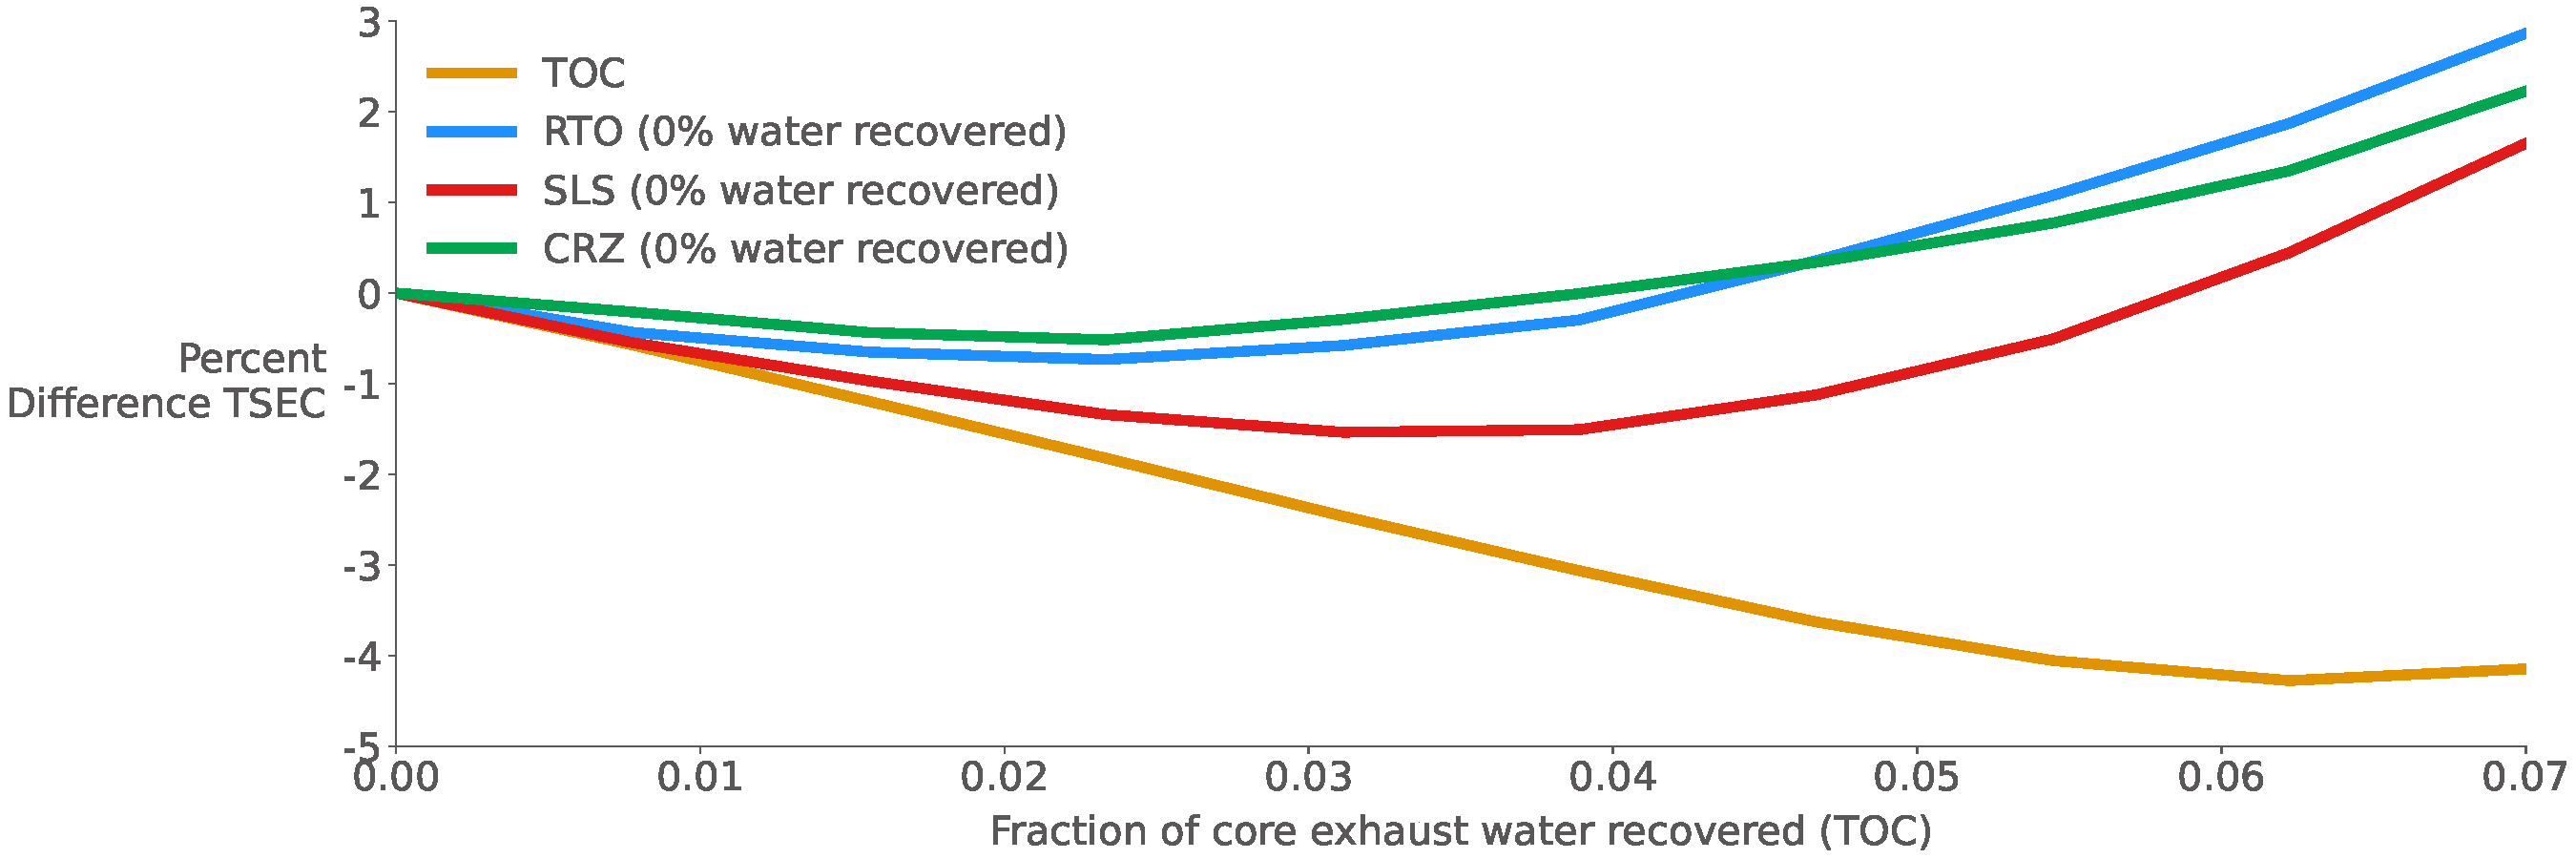
\includegraphics[width=1.0\textwidth]{TSEC_N3-CLVR-H2-0-7-TOC.pdf}
        {TOC}
    \end{minipage}
    \begin{minipage}{0.48\textwidth}
        \centering
        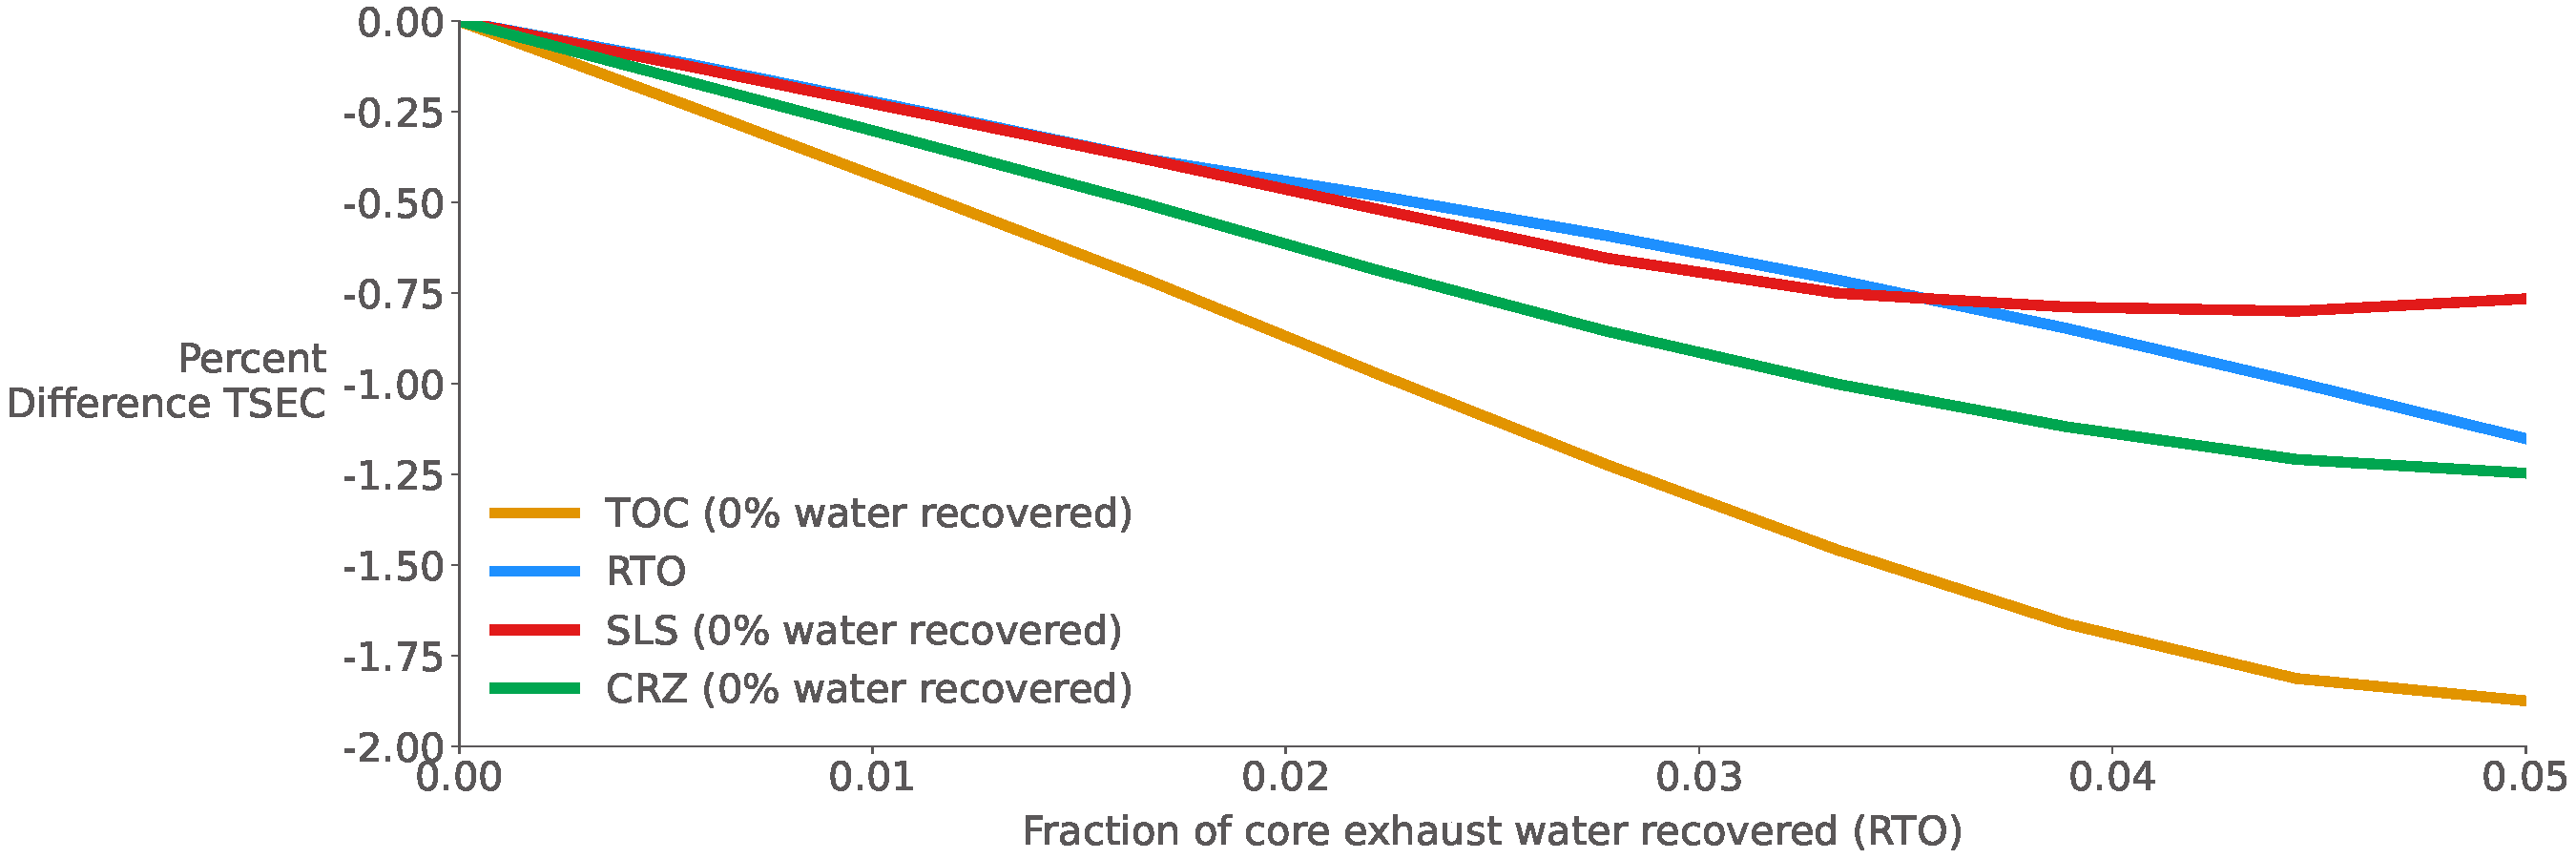
\includegraphics[width=1.0\textwidth]{TSEC_N3-CLVR-H2-0-5-RTO.pdf}
        {RTO}
    \end{minipage}
    \begin{minipage}{0.48\textwidth}
        \centering
        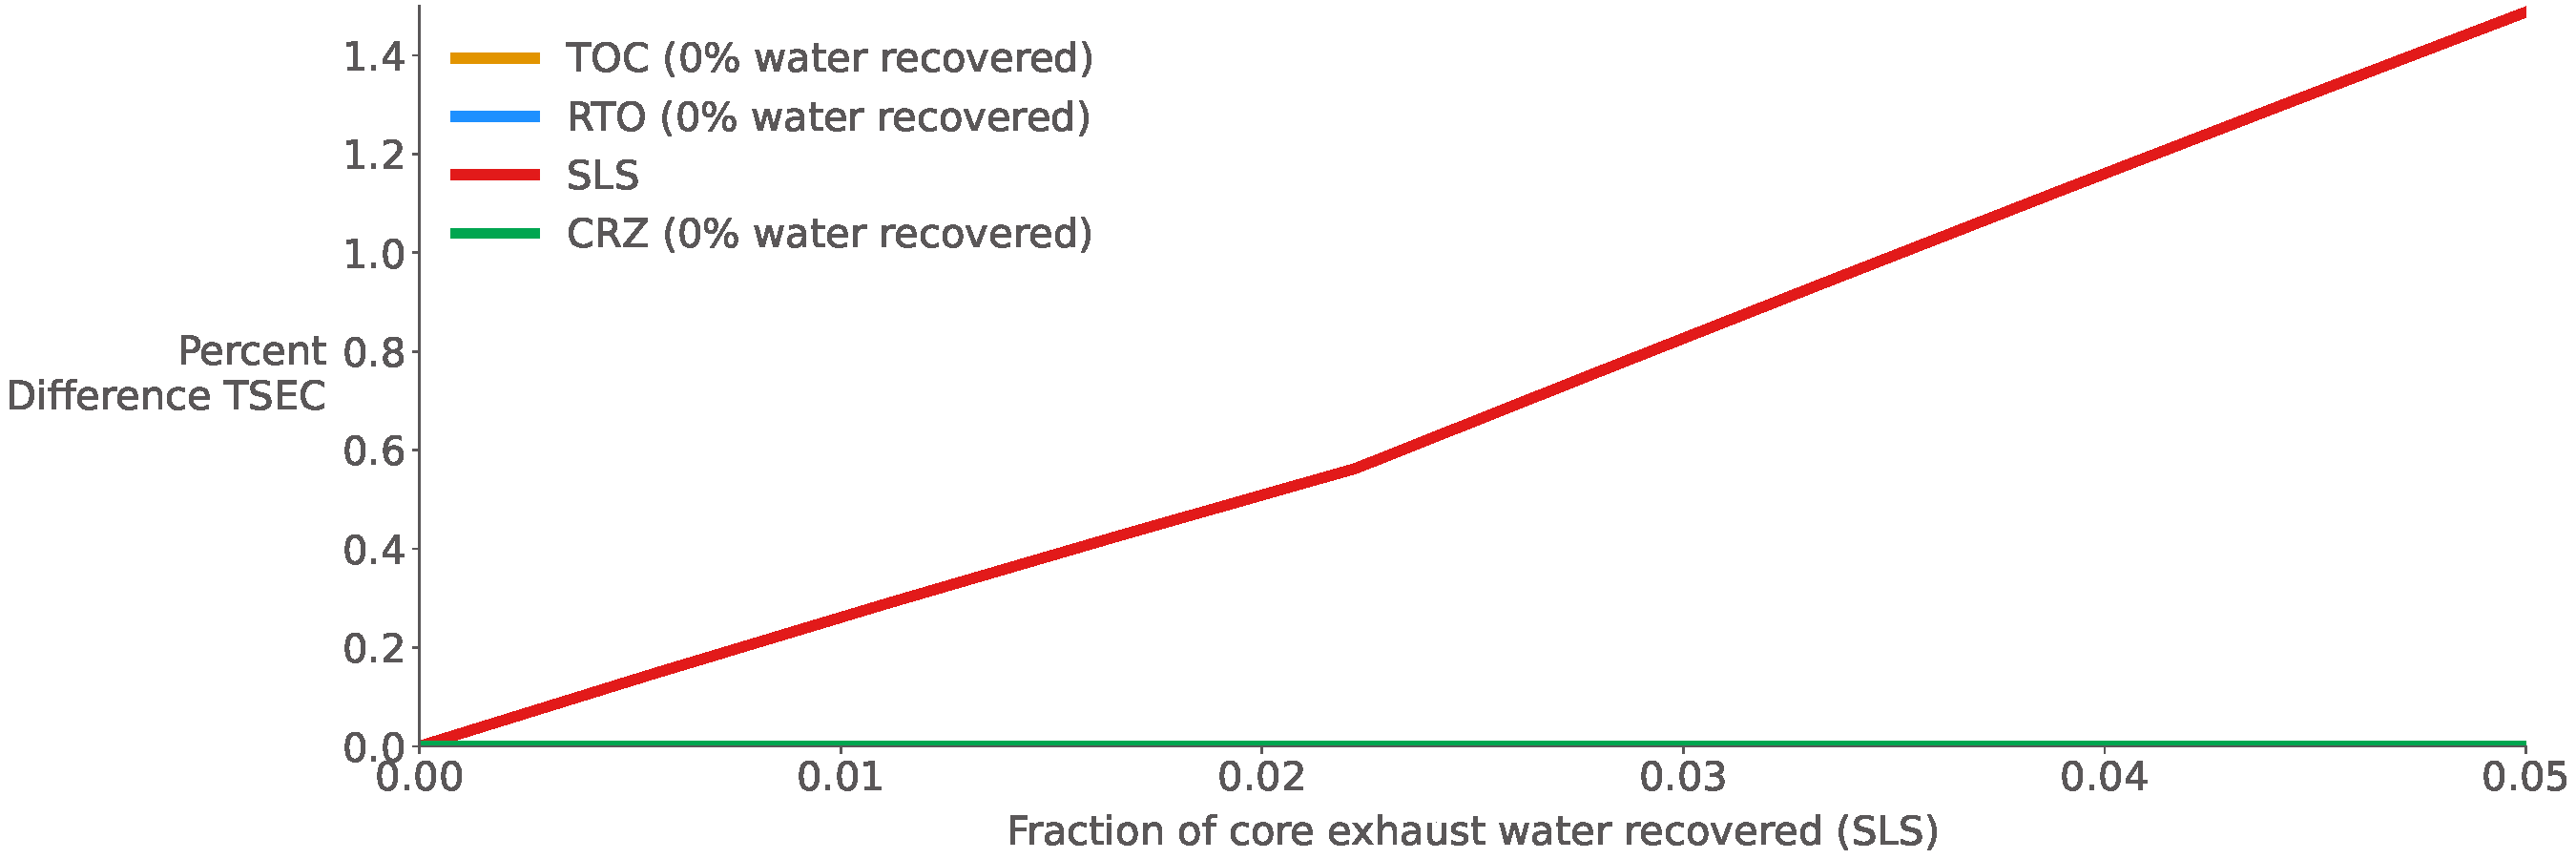
\includegraphics[width=1.0\textwidth]{TSEC_N3-CLVR-H2-0-5-SLS.pdf}
        {SLS}
    \end{minipage}
    \begin{minipage}{0.48\textwidth}
        \centering
        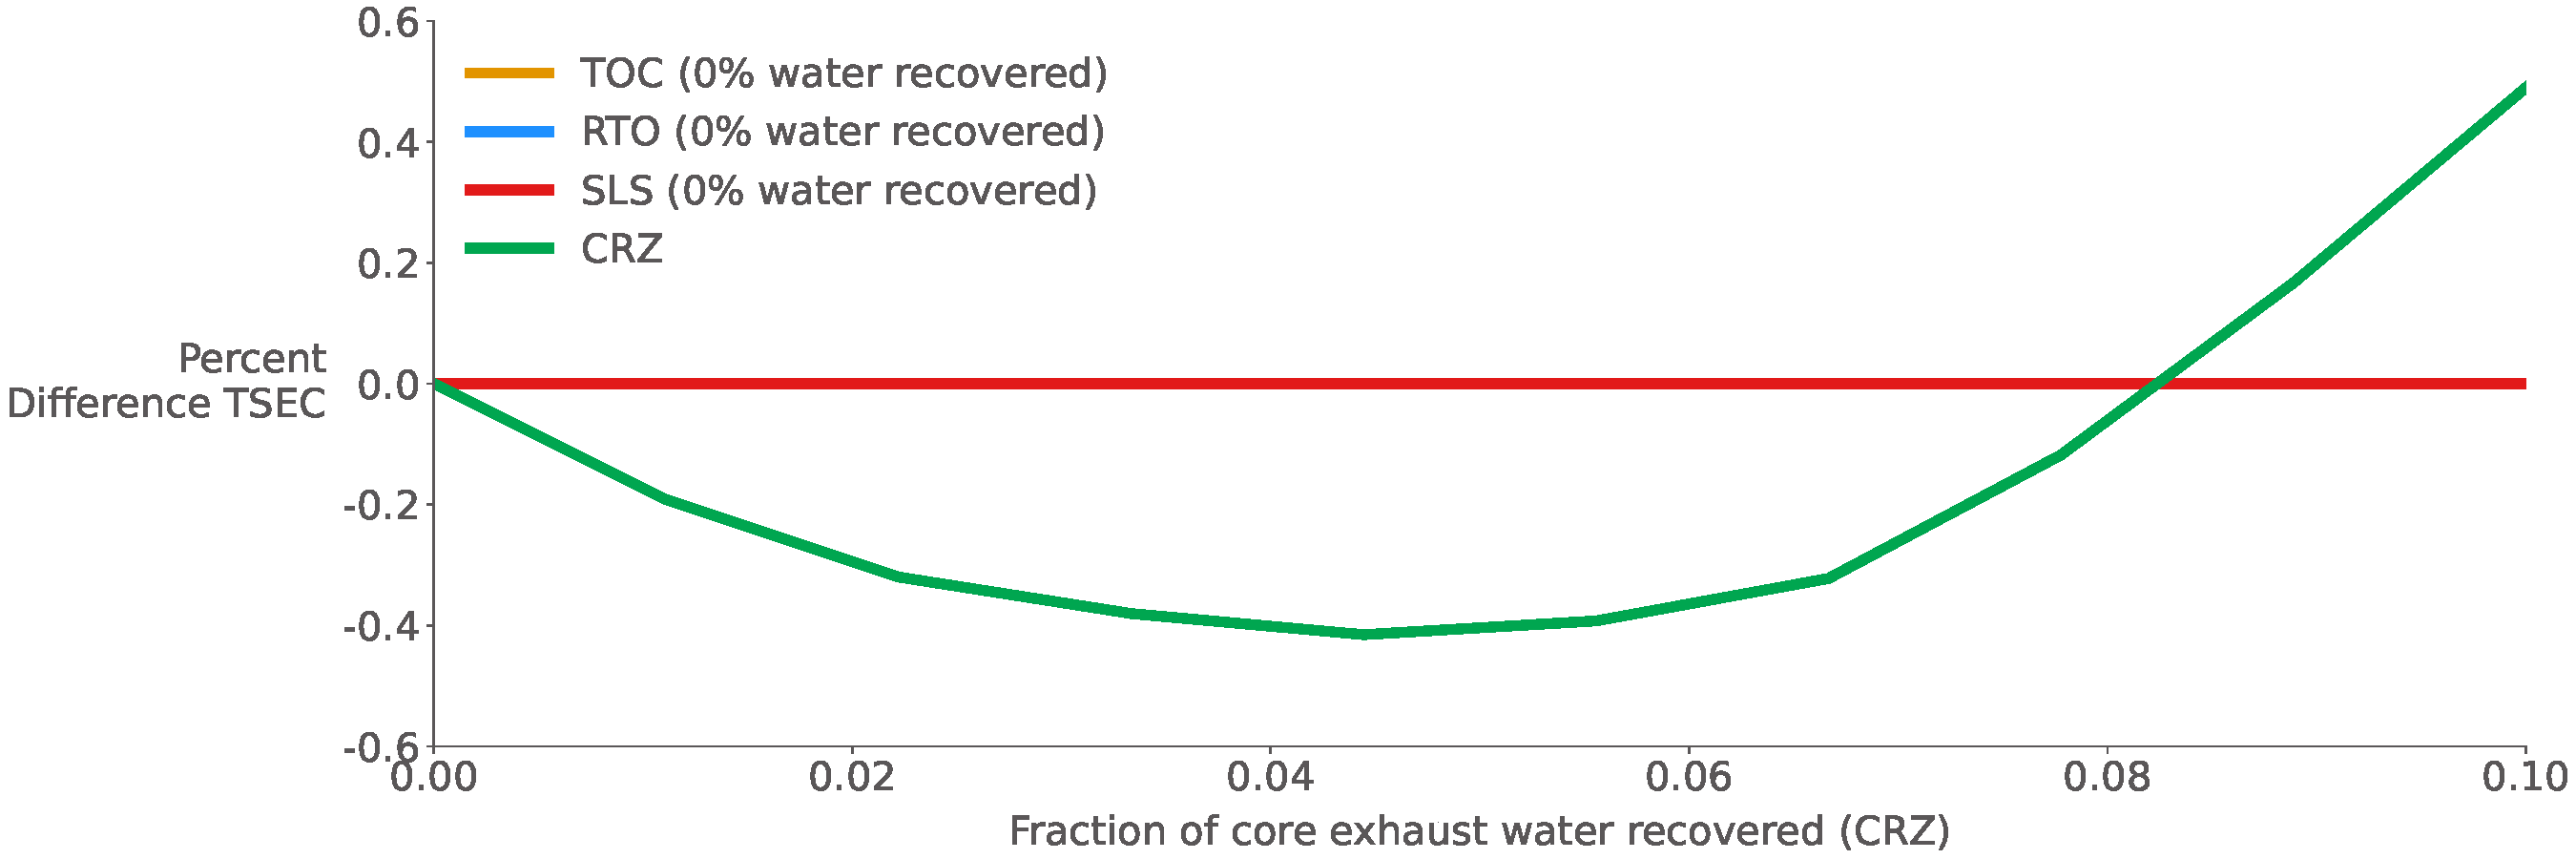
\includegraphics[width=1.0\textwidth]{TSEC_N3-CLVR-H2-0-10-CRZ.pdf}
        {CRZ}
    \end{minipage}
    \caption{}
    \label{fig:para_study}
\end{figure}

\noindent
From these figures we can see that the water fraction at TOC has a large impact on all of the off-design points. This makes sense since the design point sets the sizing of the engine and therefore dictates the performance of the off-design conditions. We also see that the water fraction at RTO has an impact on all of the operating conditions. This is due to the fact that the maximum temperature in the engine at TOC, $T_{4,TOC}$, is set by conditions at RTO. Therefore, the design point is affected by the water recovery at RTO. We see that the SLS condition has no impact on any other operating condition since its design has no impact on the other operating conditions. This is also true for the CRZ condition. The difference we see is that it is likely that the optimal water fraction at SLS will trend towards zero and the CRZ optimal water fraction will likely be non-zero.

\subsection{Optimization Problem}
The optimization problem of the N3 engine and the vapor recovery loop are shown in Figure \ref{fig:N3_xdsm_opt}.

\begin{figure}[!hbt]
    \centering
    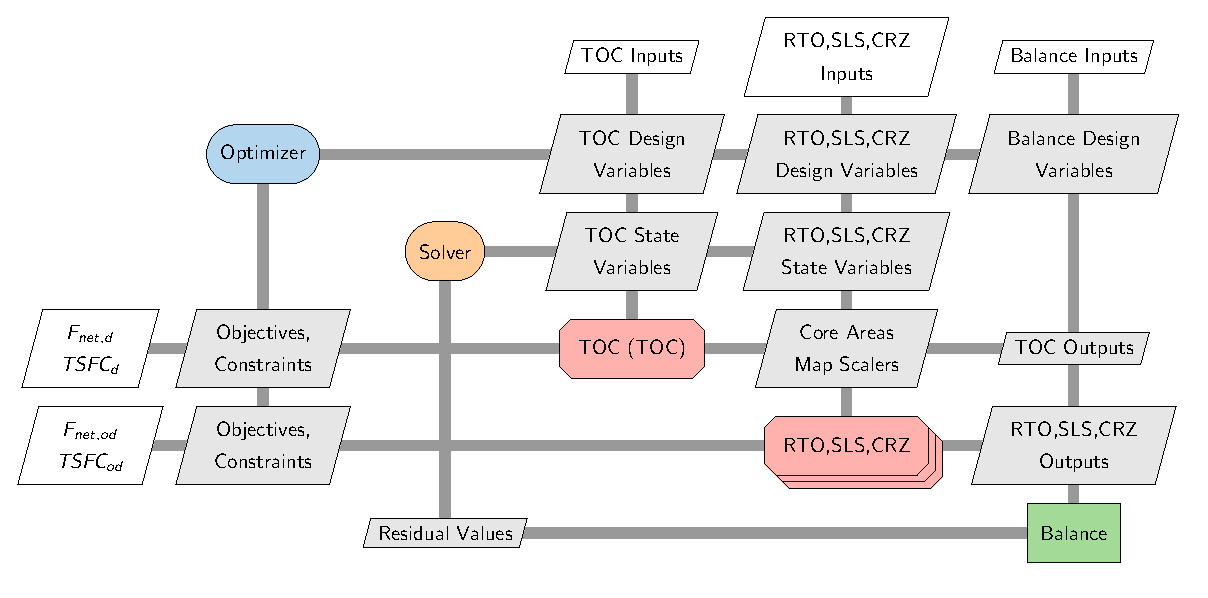
\includegraphics[width=0.75\textwidth]{N3_xdsm_opt.pdf}
    \caption{Optimization XDSM diagram.}
    \label{fig:N3_xdsm_opt}
\end{figure}

\noindent
This optimization problem was run for both JetA and H2 fuels using the parameters given in the parametric study.
The optimization problem for each fuel was specified as:

\begin{equation*}
    \begin{aligned}
         & {\text{minimize}}
         &                     & TSEC_{CRZ}                                         \\
         & {\text{by varying}}
         &                     & x_{H2O,TOC}, x_{H2O,RTO}, x_{H2O,SLS}, x_{H2O,CRZ} \\
         & \text{subject to}
         &                     & F_{net,TOC} \geq 5800 lbf                          \\
    \end{aligned}
\end{equation*}

\subsection{Optimization Results}
The SNOPT optimizations for both fuels successfully finished with a 0/1 exit code and the optimal solution is given below. Note that the water recovery fraction, $x_{H2O,CRZ}$, had to be bounded above by a specific value. This value was determined by running the optimziation until the optimizer ran into numerical issues in the model where the engine would not resolve the amount of water in the engine at the CRZ condition. The optimizer wants to keep pushing through more and more water but this eventually breaks the model. Therefore an upper bound just below the breaking point is used.

\begin{table}[H]
    \centering
    \caption{Vapor recovery loop water fraction optimization for JetA fuel.}
    \begin{tabular}{|c|c|c|c|c|c|}
        \hline
        Category    & Name          & Value   & Lower  & Upper & Units                 \\
        \hline
        Objective   & $TSEC_{CRZ}$  & 7886.58 & -      & -     & $\frac{BTU}{hr-lb_f}$ \\
        \hline
        Variables   & $x_{H2O,TOC}$ & 0.0699  & 0.0    & -     & -                     \\
                    & $x_{H2O,RTO}$ & 0.0     & 0.0    & -     & -                     \\
                    & $x_{H2O,SLS}$ & 0.0     & 0.0    & -     & -                     \\
                    & $x_{H2O,CRZ}$ & 0.27    & 0.0    & 0.27  & -                     \\
        \hline
        Constraints & $F_{net,TOC}$ & 5800.0  & 5800.0 & -     & $lbf$                 \\
        \hline
    \end{tabular}
    \label{tab_jeta_opt}
\end{table}

\begin{table}[H]
    \centering
    \caption{Vapor recovery loop water fraction optimization for H2 fuel.}
    \begin{tabular}{|c|c|c|c|c|c|}
        \hline
        Category    & Name          & Value   & Lower  & Upper & Units                 \\
        \hline
        Objective   & $TSEC_{CRZ}$  & 7840.04 & -      & -     & $\frac{BTU}{hr-lb_f}$ \\
        \hline
        Variables   & $x_{H2O,TOC}$ & 0.105   & 0.0    & -     & -                     \\
                    & $x_{H2O,RTO}$ & 0.0     & 0.0    & -     & -                     \\
                    & $x_{H2O,SLS}$ & 0.0     & 0.0    & -     & -                     \\
                    & $x_{H2O,CRZ}$ & 0.19    & 0.0    & 0.19  & -                     \\
        \hline
        Constraints & $F_{net,TOC}$ & 5800.0  & 5800.0 & -     & $lbf$                 \\
        \hline
    \end{tabular}
    \label{tab_h2_opt}
\end{table}

\noindent
The convergence plot for the JetA optimzation is shown in Figure \ref{fig:conv_opt}. The plot for H2 is similar in shape.

\begin{figure}[!hbt]
    \centering
    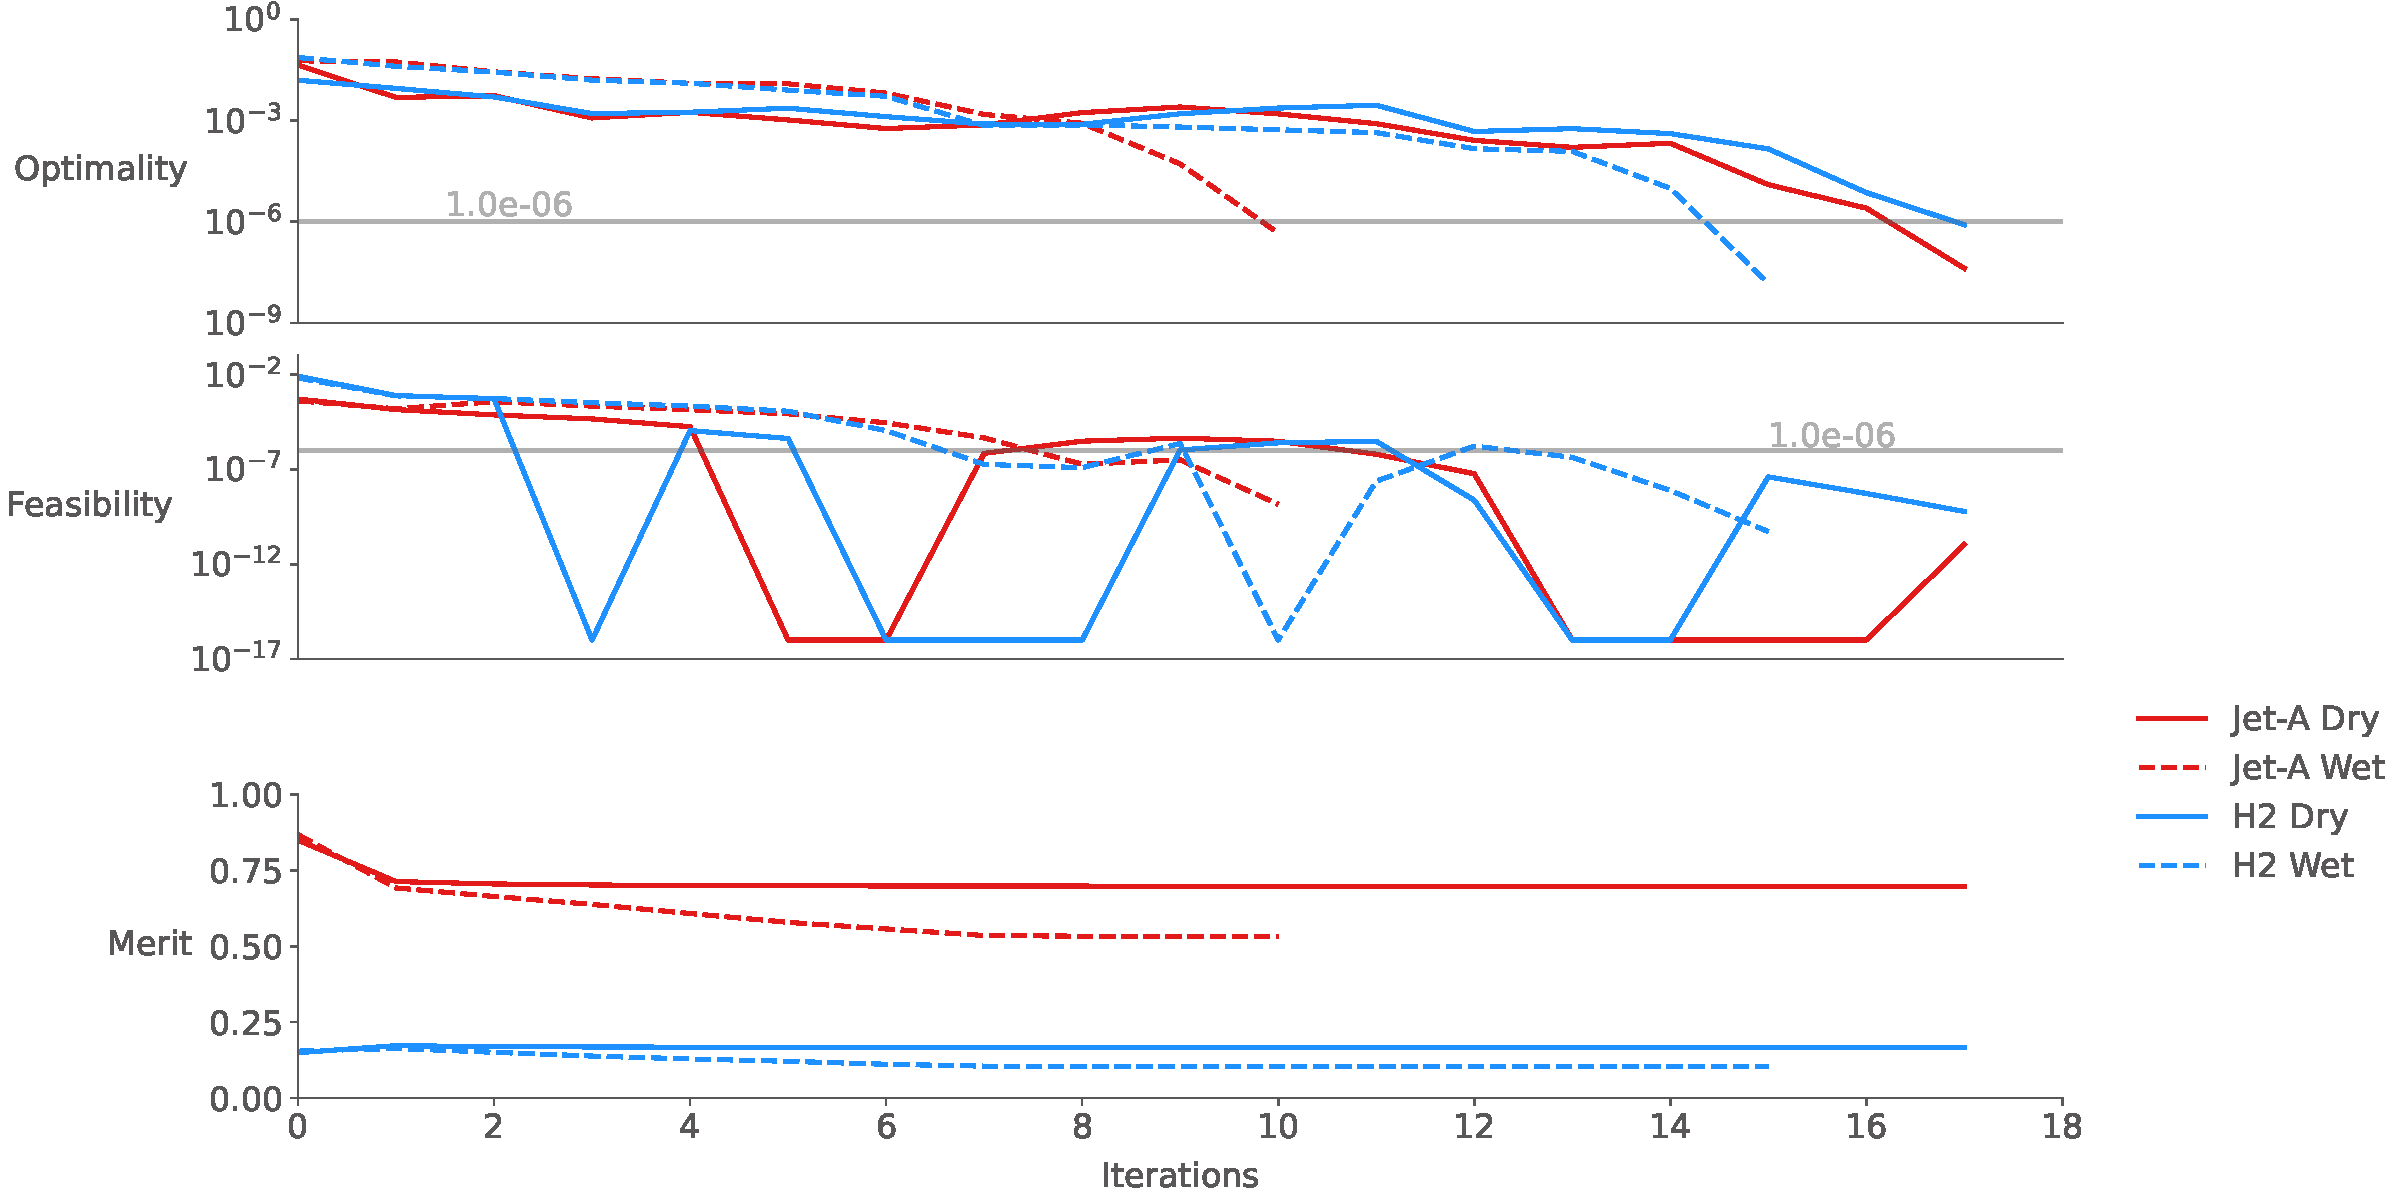
\includegraphics[width=0.75\textwidth]{opt_summary.pdf}
    \caption{Optimality and feasibility convergence plots for JetA.}
    \label{fig:conv_opt}
\end{figure}

\noindent
From these optimization problems, we can see that the in both cases the CRZ condition water recovery fraction goes all the way to the upper bound.
We also see that the TOC condtion water recovery fraction finds a non-zero point that minimizes the objective whereas the RTO and SLS conditions find the smallest possible fraction.
While we saw in the parametric studies that a non-zero $x_{H2O,RTO}$ could improve efficiency, the $x_{H2O,TOC}$ takes this into account in how it resized parts of the engine.
These optimizations show the tight coupling between the different design points.
The off-design points do not have any impact on the performance of the design point (TOC) with the exception of RTO in how it handles maximum temperatures.
When the objective is the performance of the off-design CRZ condition, then the main two tuning variables are the water fractions at TOC and CRZ since those are the only two that directly impact the objective.
Finally, we see that the H2 fuel results in a slight improvement in TSEC.
Even this slight improvement is impactful since slight improvements in fuel economy result in large carbon and cost savings, with the added bonus of the hydrogen engine producing no carbon.

\section{Conclusions}
A novel water vapor recovery loop was developed, studied, and optimized for two different types of fuel.
New pyCycle components, a water injector and water extractor, were developed for this project and implmented in the NASA N3 ultra-high bypass turbofan engine.
Additionally, nitrogen oxide emission models were introduced and implemented to allow for NOx emission constraints on the engine model.
The parametric studies that were performed show a strong coupling between the on-design and off-design operation conditions of the N3 engine.
Furthermore, the simple optimizations that were performed for each fuel show an improvement in performance with water injection and recovery.
The different fuels ended up having very similar thrust-specific energy consumption metrics with a slight improvement when using hydrogen as a fuel as opposed to the traditional JetA fuel.
These results are promising as they indicate that the efficiency improvement that has been seen in empirical results can be modeled in zero-dimensional modeling software packages such as pyCycle, allowing multidisciplinary design and analysis for future high-efficiency engine and aircraft design.
Future plans for this project are to use this model to run large parallel sweeps of the model design space and to eventually create a surrogate model of this engine for use in other optimization libraries such as OpenConcept.
Additionally, water condensor models may be researched in the future so that a fairly accurate condensor and pressure loss model can be implemented for the extractor to determine how severe the pressure loss penalties are.
Finally, a pareto front will be computed to determine the tradeoffs between TSEC and NOx emissions for the JetA fuel.
All of these future studies will help determine if the claims of performance enhancements and emission reductions of water recovery and hydrogen engines that are promoted by industy are within the realm of possibliy.

\bibliography{mdolab,references}

% \newpage

% \section*{Appendix: Compressor and Turbine Maps}

% \begin{figure}[H]
%     \centering
%     \includegraphics[width=0.75\linewidth]{TOC.fan.pdf}
%     \caption{Optimized engine location on the fan map (black dot).}
%     \label{}
% \end{figure}

% \begin{figure}[H]
%     \centering
%     \includegraphics[width=0.75\linewidth]{TOC.lpc.pdf}
%     \caption{Optimized engine location on the low pressure compressor map (black dot).}
%     \label{}
% \end{figure}

% \begin{figure}[H]
%     \centering
%     \includegraphics[width=0.75\linewidth]{TOC.hpc.pdf}
%     \caption{Optimized engine location on the high pressure compressor map (black dot).}
%     \label{}
% \end{figure}

% \begin{figure}[H]
%     \centering
%     \includegraphics[width=0.75\linewidth]{TOC.lpt.pdf}
%     \caption{Optimized engine location on the low pressure turbine map (black dot).}
%     \label{}
% \end{figure}

% \begin{figure}[H]
%     \centering
%     \includegraphics[width=0.75\linewidth]{TOC.hpt.pdf}
%     \caption{Optimized engine location on the high pressure turbine map (black dot).}
%     \label{}
% \end{figure}

\end{document}
